
 \chapter{Metodología de Desarrollo}
 \label{cha:metodologia_de_desarrollo}

\section{Introducción}

   La metodología para el desarrollo de software permite gestionar y administrar un proyecto de desarrollo de software para llevarlo a término de una forma más eficiente y con altas probabilidades de éxito, seguir una metodología es importante ya que ayudará a organizar y a seguir un ritmo de trabajo.

  %  Para este proyecto de grado se hará uso de una metodología Ágil, por lo cual se definirá en que se basan las metodologías ágiles.

   % Para este proyecto de grado se va a ser uso de \emph{XP} como metodología ágil.\\

   \section{Metodologías Ágiles}
   \label{sec:metodologias_agiles}

   Este término nace en una reunión celebrada en febrero de 2001 en Utah - USA por expertos en la industria del software ya que pretendían encontrar una forma alternativa de desarrollo de software a las que estaban vigentes hasta esa fecha por ejemplo la metodología en cascada que es rígido y obliga una planeación extensiva antes siquiera de tocar una línea de código, está demostrado que este tipo de metodologías son muy rígidas y les falta flexibilidad a la hora de hacer frente a los cambios que invariablemente sufre un proyecto de desarrollo de software.\\

   % //·        In reality it is very difficult for projects to follow the sequential flow of the model
   % //·        It is difficult to identify all requirements and goals at the beginning of projects as requirements tend to change all the way
   % //·        A working version can only be obtained late in the process


   Para contravenir estas dificultades es que se definieron los principios del manifiesto ágil\footnote{\url{http://agilemanifesto.org/iso/es/manifesto.html}}:

   \begin{quote}
     \begin{description}
       \item[Individuos e interacciones] sobre procesos y herramientas.
       \item[Software funcionando] sobre documentación extensiva.
       \item[Colaboración con el cliente] sobre negociación contractual.
       \item[Respuesta ante el cambio] sobre seguir un plan.
       % \cite{agile_manifesto}
     \end{description}
   \end{quote}

   % The main concern of agile methodologies is the ability to embrace changes which are very likely to happen in environments which lack predictability [6]

   El principal objetivo de las metodologías ágiles es la habilidad de soportar los cambios, los cuales generalmente por no decir casi siempre aparecen en un ambiente que sufre muchos cambios y rápidamente, los cuales son difíciles de predecir.\cite{design2005}

   % //To achieve the objective, agile methodologies use three key principles [8]: (1) a focus on adaptive methodologies, (2) a focus on people, and (3) a focus on self-adaptive processes.

   Para alcanzar este objetivo es que las metodologías ágiles se basan en tres principios: \cite{xpHutagalung}

\begin{itemize}
 \item Enfoque en metodologías que se adapten al cambio
 \item Enfocarse en las personas
 \item Enfocarse en procesos que se auto-adapten al cambio
\end{itemize}

   Las metodologías ágiles no se refieren a un único y específico metodo o tecnica de desarrollo, en cambio son un grupo de metodologías que implementan los principios ágiles. Entre los cuales se pueden apreciar las siguiente metodologías:

   \begin{itemize}
     \item Scrum
     \item Dynamic Systems Development Method (DSDM)
     \item Crystal Methods
     \item Feature Driven Development
     \item Lean Development
     \item Extreme Programming (XP)
     \item Adaptive Software Development
   \end{itemize}


   % Por las siguientes características de la Metodología \emph{Programación eXtrema}, la cual viene del inglés \emph{eXtreme Programing} por lo cual generalmente se referirá a esta como \emph{XP} y es la que es la escogió para implementar este proyecto de grado.


   % End metodologias_agiles


   \section{Programación Extrema}
   \label{sec:xp}

     La \emph{programación extrema} o \emph{XP} es una metodología de trabajo creada a mediados de 1990 por Kent Beck cuando estaba trabajando en un proyecto de desarrollo de software en \emph{Chrysler Comprehensive Compensation} (C3) en un intento de mejorar el proceso de desarrollo de software y posteriormente con una segunda implementación de un proyecto usando la metodología XP en \emph{Vehicle Cost and Profitability System (VCAPS)} propiedad de \emph{Ford Motor Co}, se demostró que esta metodología de desarrollo es un método apropiado para llevar a buen término el proyecto de desarrollo de software. \cite{xp_site}

     \emph{XP} se enfoca en la adaptabilidad ya que el desarrollo de software debería ser un proceso fluido donde los requerimientos no pueden ser totalmente predichos desde el principio del desarrollo ya que estos siempre o casi siempre tienden a cambiar a medida que el software se va desarrollando ya sea por cambios en el mercado o a medida que el cliente va aprendiendo y modificando sus requerimientos en el transcurso del ciclo de desarrollo del producto.

     Kent Beck declaró los siguientes cuatro enunciados que son la base de la filosofía de XP:

     \begin{itemize}
       \item Es necesario mejorar la comunicación
       \item Es necesario encontrar simplicidad
       \item Es necesario obtener feedback o retroalimentación de parte del cliente
       \item Es necesario proceder con coraje.
     \end{itemize}

     Combinando estos principios, la programación extrema se trata acerca de mejorar el trabajo en equipo cohesionado y con la ayuda de la retroalimentación propia del equipo se puede apreciar donde se encuentra y mejorarlo, siempre tomando en cuenta que cada equipo es único, ya sea por el tipo de software que se está desarrollando y por las personas que conforman el equipo.

     Las prácticas usadas en XP son de hecho prácticas comúnmente usadas en las metodologías ágiles pero en XP estas prácticas son llevadas al extremo de ahí el nombre de programacion extrema.

     La programación extrema se caracteriza por las siguiente practicas: \cite{xpesp}

     \begin{itemize}
       \item \textbf{Code reviews:} O revisión de código, en programación extrema esto se llama programación en pareja (pair programing), esto significa que dos programadores escriben código usando o compartiendo una máquina, esto se traduce en que el código es constantemente revisado y por lo tanto es menos proclive de producir errores.

       \item \textbf{Testeo:} En XP significa hacer unit testing o pruebas unitarias durante todo el proceso de desarrollo de software, una vez el producto es entregado al cliente este se encarga de probar la funcionalidad del sistema.

       \item \textbf{Diseño:} En XP se necesita que todos los involucrados en el proyecto estén siempre y constantemente refactorizando y mejorando el producto.
       Simplicidad: Siempre dejar el sistema con el diseño más simple posible para que soporte la funcionalidad deseada o lo más simple que funciona. Se basa en la filosofía de que el mayor valor de negocio es entregado por el programa más sencillo que cumpla los requerimientos.

       \item \textbf{Arquitectura:} Todos trabajando definiendo y redefiniendo constantemente la arquitectura del sistema.
       Testeo de integración: Unir o integrar y probar las diferentes características del software que se están trabajando, constantemente o por lo menos una vez al dia.

       \item \textbf{Iteraciones cortas:}
       Trabajar en ciclos realmente cortos, puede ser de horas o días pero no semanas o meses, permitiendo que el programa, el verdadero valor del negocio, pueda ser evaluado.

       \item \textbf{Propiedad colectiva del código:}
       un código con propiedad compartida. Nadie es el propietario de nada, todos son el propietario de todo. Este método difiere en mucho a los métodos tradicionales en los que un simple programador posee un conjunto de código.

       \item \textbf{Estándar de codificación:} define la propiedad del código compartido así como las reglas para escribir y documentar el código y la comunicación entre diferentes piezas de código desarrolladas por diferentes equipos

       \item \textbf{Bienestar del programador:} La semana de 40 horas, la programación extrema sostiene que los programadores cansados escriben código de menor cualidad. Minimizar las horas extras y mantener los programadores frescos, generará código de mayor calidad.

     \end{itemize}


     \subsection{Las historias de usuario}
     \label{sub:user_story}


     Es la técnica que utiliza XP para especificar los requisitos del software. Se trata de tarjetas en las cuales el cliente escribe las características que el sistema debe poseer, sean requisitos funcionales o no funcionales. El proceso de manejar las historias de usuario es muy dinámico ya que se pueden añadir, eliminar o modificarse de acuerdo a la exigencia que puede aparecer a cualquier momento, las historias deben ser lo bastante simples como para que los programadores las implementen en unas semanas.\cite{xpesp}
     % end user_story

     \subsection{Proceso de desarrollo}
     \label{sub:proceso_desarollo}

     La programación extrema identifica las siguientes fases en el proceso de desarrollo de software. \cite{xpesp}

     \begin{itemize}

       \item \textbf{Interacción con el cliente:}
       El cliente es una parte importante en el equipo de desarrollo, tiene gran importancia en el equipo ya que expresa su opinión sobre el producto después de cada cambio o iteración, mostrando las prioridades y expresando su opinión sobre los problemas que se podrían identificar.

       \item \textbf{Planificación del proyecto:}
       En este punto se se elabora la planificación por etapas o iteraciones. Para hacerlo será necesaria la existencia de reglas que han de seguir las partes implicadas en el proyecto.

       \item \textbf{Diseño, desarrollo y pruebas:}
       El desarrollo es la parte más importante en el proceso de la programación extrema. Todos los trabajos tienen como objetivo que se programen lo más rápidamente posible, sin interrupciones y en la dirección correcta.

     \end{itemize}


     %end proceso_desarollo


     \subsection{Roles de la programación extrema}
     \label{sub:roles_xp}

     Los roles de la programación extrema que fueron implementados en el presente proyecto fueron:

     \begin{itemize}
       \item \textbf{Programador:} Escribe las pruebas unitarias y produce el código del sistema.
       \item \textbf{Cliente:} Escribe las historias de usuario y las pruebas funcionales para validar su implementación. Asigna la prioridad a las historias de usuario y decide cuáles se implementan en cada iteración centrándose en aportar el mayor valor de negocio.
       \item \textbf{Tester:} Ayuda al cliente a escribir las pruebas funcionales. Ejecuta pruebas regularmente, difunde los resultados en el equipo y es responsable de las herramientas de soporte para pruebas.
       \item \textbf{Tracker:} Es el encargado de seguimiento. Proporciona realimentación al equipo. Debe verificar el grado de acierto entre las estimaciones realizadas y el tiempo real dedicado, comunicando los resultados para mejorar futuras estimaciones.
       \item \textbf{Entrenador (coach):} Responsable del proceso global. Guía a los miembros del equipo para seguir el proceso correctamente.
       \item \textbf{Consultor:} Es un miembro externo del equipo con un conocimiento específico en algún tema necesario para el proyecto. Ayuda al equipo a resolver un problema específico.
       \item \textbf{Gestor (Big boss):} Es el dueño de la tienda y el vínculo entre clientes y programadores. Su labor esencial es la coordinación.
     \end{itemize}


     % end roles_xp

     \section{El Proceso XP} % (fold)
     \label{sec:Proceso XP}

    %  Ya que para el desarrollo del proyecto se usará programación extrema,
    %  se va a definir el proceso de desarrollo general que se usará en este proyecto de grado.\\
     %
    %    % \section{Proceso de Desarrollo}
       % \label{sec:proceso_de_desarrollo}

       XP propone un proceso iterativo e incremental, El proyecto es dividido en pequeños “mini-proyectos”, los cuales terminan con un \emph{release} que es una versión del producto que se libera al final de un ciclo de desarrollo de software, un \emph{release} contiene requerimientos implementados, tal vez no acabados en un  100\% pero funcional de tal forma que el cliente es capaz de ofrecer \emph{feedback} del producto. \cite{xp_overview}

       Estos ``mini-proyectos'' o iteraciones, son negociados entre los clientes y los desarrolladores, donde el cliente determina el valor de negocio de las características que se quiere desarrollar y los desarrolladores especifican el tiempo y esfuerzo que se necesita para desarrollar estas características, el cliente sopesa el valor, el esfuerzo y el tiempo de la iteración y decide qué características se desarrollaran, como último paso en la iteración los desarrolladores implementan las características seleccionadas.

     % En un proyecto que sigue la metodología XP los releases son frecuentes, esto para recibir feedback más seguido. Los releases son negociados en un Planning Game, donde los clientes definen qué se va a implementar en el release y los desarrolladores especifican el tiempo que necesitan para desarrollar las características deseadas.\\

           En la figura \ref{fig:xp_diagram} se puede apreciar el diagrama del proceso de desarrollo de la metodología XP.


     \begin{figure}[H]
       \begin{center}
         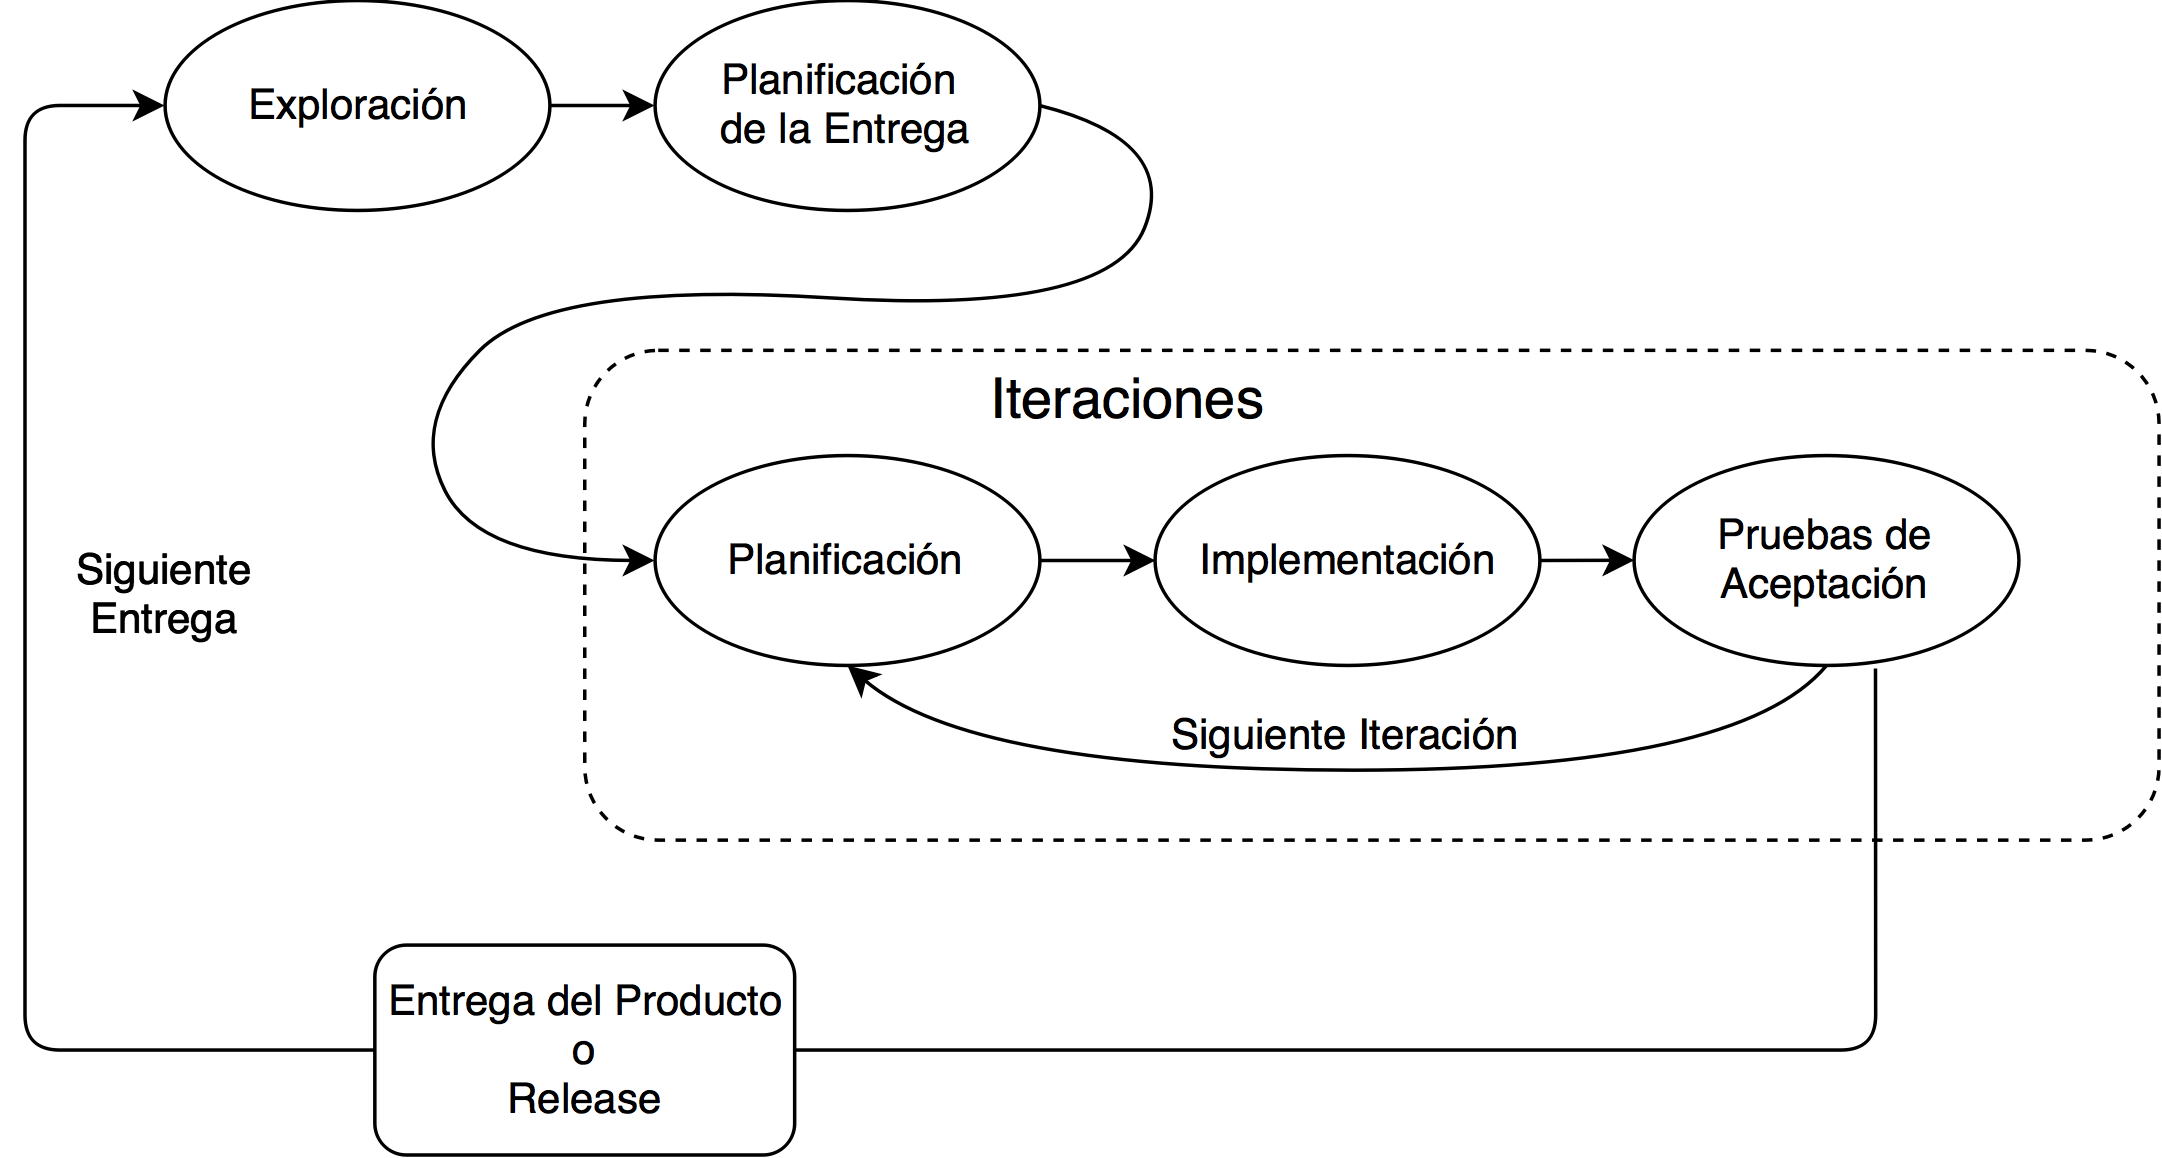
\includegraphics[width=1\textwidth]{xp_diagram}
         \caption{Diagrama del proceso XP}
         \label{fig:xp_diagram}
         % \caption*{Fuente: \cite{xp_overview}}
         \caption*{Fuente: Implementación propia}
       \end{center}
     \end{figure}



       \subsection{Exploración}
       \label{sub:Exploracion}

       Es la primera fase, durante la cual los clientes definen lo que desean que tenga el sistema y los desarrolladores estiman el tiempo necesario que necesitan para realizar esas tareas.
       % La fase del planning game consiste de 3 etapas: exploración, planeacion y direccion.\\

       % Durante la fase de la \emph{exploración} los clientes definen lo que desean que tenga el sistema y los desarrolladores estiman el tiempo necesario que necesitan para realizar esas tareas.\\
       %
       % Durante la \emph{planeación} se negocia y se decide cuales de todas las características que los clientes quieren pueden llegar a realizarse en el tiempo dise~ado para una iteración.\\
       %
       % Después de la planeación sigue la fase de \emph{dirección}, durante la cual se desarrolla y actualiza (cuando sea necesario) la planeación ya negociada según lo que se vaya aprendiendo a medida que avanza el desarrollo del proyecto.\\

         % \subsubsection{Exploración}
         % \label{subs:exploracion}

           Durante esta etapa el cliente escribe las tarjetas de \emph{historias de usuario}, estas historias definen lo que el cliente quiere que el sistema haga, en otras palabras representan las características que el sistema debería tener implementado.

           Es gracias a las \emph{historias de usuario}, que el equipo de desarrollo comienza a aprender de las herramientas y las tecnologías que va a utilizar, para posteriormente  asignar una estimación de tiempo y esfuerzo que necesitará el desarrollo de las \emph{historias del usuario}.

         % end exploracion

         \subsection{Planificación de la Entrega}
         \label{sub:planeacion}

       Cuando se tienen las historias de usuario, el cliente determina la prioridad y los desarrolladores estiman el esfuerzo necesario para cada una, se procede a una negociación donde se aceptan qué historias se van a desarrollar en primer lugar y en cuanto tiempo se entregaran resultados, en esta etapa se define el ``plan de entregas''.

% se está listo para una “negociación de aceptación” donde un “calendario de entregas”  es negociado y

       Las historias de usuario se las crea para propósitos de planeación y estimación de tiempo y esfuerzo que cada característica va a necesitar, los detalles se crean y dividen posteriormente en las \emph{tareas de ingeniería} cuando las historias están por ser implementadas.


       % Durante esta fase el cliente escoge las historias de usuario que serán implementadas en la presente iteración, generalmente se escogen las que aportan más valor al producto o tienen más relevancia en la lógica de negocio del cliente, asi como tambien cualquier historia que no se acabó en una iteración anterior.\\
       %
       % Los desarrolladores dividen las historias en Tareas de Ingeniería, las cuales son más pequeñas que las historias, si se encuentra que una Tarea es casi tan grande como una historia es porque es una historia y debería ser dividida en Tareas. Una tarea puede estar relacionada a 2 o mas historias o no estar relacionada con ninguna historia. Dentro de la metodología XP es una buena práctica el escribir las tareas en las  “Index Cards”, similares a las historias, esto debido a que estas tarjetas son fáciles de manipular durante la fase de planeación.\\


         % end planeacion

         % \subsubsection{Iteraciones}
         % \label{subs:Iteraciones}
         %
         % Esta fase es básicamente comprende el resto del desarrollo del producto hasta que es liberado al mercado o el proyecto es cancelado.\\
         %
         % Esta fase consiste en 4 ``movimientos'':
         %
         % \begin{itemize}
         %   \item \textbf{Iteración:} Es durante la iteración cuando se desarrolla el producto, el tiempo que se utiliza para esta fase es de generalmente de una o 2 semanas, dependiendo de la naturaleza del proyecto.
         %
         %   \item \textbf{Recuperación:} Si durante el desarrollo no se completan las características a desarrollar en el tiempo establecido, es durante la recuperación que se re-negocia con el cliente si quiere cambiar la fecha de entrega del release o modificar el alcance del desarrollo (menos historias de usuario).
         %
         %   \item \textbf{Nuevas Historias:} El cliente tiene el derecho de aumentar historias de usuario, las cuales se tienen que estimar y negociar si serán parte del actual desarrollo, en tal caso se tiene que renegociar las fechas de entrega.
         %
         %   \item \textbf{Re-estimación:} Si durante el desarrollo el equipo considera que el plan ya no es correcto, todas las historias que faltan hacer se tienen que re-estimar y el plan se tiene que re-negociar con el cliente.
         % \end{itemize}

       % end planning_game

         \subsection{Iteraciones}
         \label{sub:iteracion}

           % \subsubsection{Iteración}
           % \label{subs:iteracion}
           %
           % La fase de Iteración en XP se lo denomina como \emph{Iteration Planning Game}, esta al igual que  el release planning game consiste en las fases de: Exploración, Planeacion e Implementacion.\\

           Esta fase es un conjunto de iteraciones de entre 2 y 3 semanas, cada iteración consta de las siguientes etapas: Planificación, Implementación y Pruebas de Aceptación.

           %
          %  \begin{itemize}
          %    \item \textbf{Planificación:}

           \subsubsection{Planificación}


           Cada iteración tiene su propia etapa de \emph{planificación} donde se tienen en cuenta las historias de usuario seleccionadas, las faltantes y las tareas que se realizarán.

             Los desarrolladores dividen las historias de usuario en \emph{Tareas de Ingeniería}, las cuales son más pequeñas que las historias, si se encuentra que una \emph{Tareas de Ingeniería} es casi tan grande como una historia de usuario es porque es una historia de usuario y debería ser tratada como tal.

             Una tarea puede estar relacionada a 2 o mas historias o no estar relacionada con ninguna. Dentro de la metodología XP es una buena práctica el escribir las tareas en tarjetas, similares a las historias de usuario, esto debido a que las tarjetas son más fáciles de manipular.

             Durante esta fase un desarrollador acepta la responsabilidad de implementar una \emph{Tarea de Ingeniería} de acuerdo de su experiencia personal en el área y tecnologías que se usarán en el desarrollo. El desarrollador debe estimar el tiempo necesitado para completar la tarea en un Tiempo de Ingenieria Ideal, una regla de XP consiste en que no se debe realizar trabajo el cual no se va necesitar en ese momento, \textbf{YAGNI}\footnote{You aren't gonna need it. En español, Tu no lo vas a necesitar o No vas a necesitarlo.}.


             \subsubsection{Implementación}
            % \item \textbf{Implementación:}

            Durante esta etapa el equipo de desarrollo empieza a escribir codigo que satisfaga los criterios de aceptación descritos en la \emph{Historia de Usuario} seleccionada para ser trabajada en la Iteración, \emph{XP} propone los siguientes procedimientos:

              % Es durante esta etapa que el equipo de desarrollo analiza las tareas de ingeniería asignadas y procede a implementar el codigo suficiente para satisfacer el criterio de aceptación descrito en la historia de usuario relacionada, la metodología \emph{XP} propone los siguientes procedimientos:

              \begin{itemize}
                \item Analizar lo que hay que hacer, esto envuelve lo que es analizar las \emph{Tarjetas de Ingeniería} y/o las \emph{Historias de Usuario}. %, de ser necesario se realiza una sesión CRC.

                \item Escribir Pruebas Unitarias, son bastante útiles para determinar cuando la tarea está completada.

                \item Implementar el código suficiente para lograr que las pruebas unitarias pasen exitosamente.

                \item Simplificar el código si es necesario (\emph{Refactor Mercilessly}).

                \item Integrar los cambios continuamente (\emph{Continuous Integration}).

              \end{itemize}
              % end implementacion

\subsubsection{Pruebas de Aceptación}
% \item \textbf{Pruebas de Aceptación:}
              Cada \emph{Historia de Usuario} lleva asociado pruebas, estas son diseñadas para verificar que los criterios de aceptación de cada \emph{Historia de Usuario} fueron implementadas correctamente. Si durante esta fase las pruebas fallan, la historia de usuario relacionada se marca para volver a trabajarla en la siguiente iteración.\\


              Las pruebas de aceptación son escritas y ejecutadas para validar la calidad del producto que se está entregando, hay que subrayar que ningún producto o aplicación desarrollado está exento de fallas, porque los que escriben los programas son personas y las personas siempre tienden a cometer errores. \\

              Es por esta razón que las pruebas de aceptación son de gran importancia porque ayudan a detectar las fallas o posibles fallas que el sistema puede tener. La detección temprana de errores es de gran importancia en el desarrollo de software ya que los errores encontrados en etapas de implementación son más baratos que los errores encontrados por el cliente, estos errores cuestan más porque socavan la confianza  del cliente o usuario hacia el producto desarrollado. \\

              Tomando en cuenta los alcances demarcados para el presente proyecto se hará énfasis en los siguiente criterios de calidad durante la fase de Iteración.


              %
              % Las pruebas de aceptacion buscan validar distintos criterios de calidad, y para el presente proyecto se hara enfacis en los criterios de funcionalidad, usabilidad y rendimiento,


              \begin{itemize}
                \item \textbf{Funcionalidad:} Las \emph{pruebas funcionales}, son diseñadas tomando como referencia las especificaciones funcionales de un componente o sistema, sirven para comprobar si el software cumple las funciones esperadas. Estas pruebas están comprendidas en lo que se denominan \emph{pruebas de caja negra}. \cite{glosarioTesting} \\

                Dentro de las pruebas funcionales se pueden encontrar 2 tipos de pruebas, las pruebas positivas y  las pruebas negativas.  Las \emph{pruebas positivas} se caracterizan por usar datos de entrada válidas y así comprobar que el sistema funciona como espera el usuario. Las \emph{pruebas negativas} usan datos de entrada no-válidas o negativas esperando un error como resultado, el cual sea el esperado en relación a la funcionalidad del sistema. \cite[p. 24]{casosPruebaUmss}


                \item \textbf{Usabilidad:} El objetivo del atributo de usabilidad es lograr
              que al usuario le sea cómoda y fácil la operación como también el manejo de la aplicación, las aplicaciones que no son usables son fácilmente cambiadas por aplicaciones que cumplen esta característica.  \cite[p. 27]{qaWeb}


              \end{itemize}




              Es buena práctica ejecutar todas las pruebas escritas al final de cada iteración, \emph{pruebas de regresión}, de esta forma se puede comprobar que durante la implementación de código durante la presente iteración no se haya roto la funcionalidad de las características ya implementadas en anteriores iteraciones. \cite[p. 25]{metodosAgiles}




          %  \end{itemize}

          \subsection{Producción}
          \label{sub:produccion}

          En la fase de producción se realizarán pruebas para validar el correcto funcionamiento del sistema en general, \emph{pruebas de rendimiento}, como resultado de estas pruebas se evalúa que el software desarrollado cumple con las características mínimas acordadas para su entrega al cliente. \cite[p. 139]{casosPruebaUmss} \\

         %  Las pruebas que se realizarán durante esta fase serán las \emph{Pruebas No Funcionales}, las pruebas no funcionales son pruebas que no se refieren a las funcionalidades, sinó a atributos transversales a la misma, como la usabilidad, la mantenibilidad, la eficiencia, etc. \cite{glosarioTesting} \\

         % Los tipos de pruebas de rendimiento son: pruebas de carga, pruebas de estrés, pruebas de resistencia
         % Dentro de las pruebas de rendimiento son bastante amplias y de

         Tomando en cuenta que se desarrollara una aplicación web, se utilizarán \emph{pruebas de carga} para validar el rendimiento de la aplicación.

         \begin{itemize}
           \item \textbf{Pruebas de Carga:} Este tipo de prueba es realizado para evaluar el comportamiento de los componentes del sistema con un incremento de carga constante, por ejemplo una cantidad determinada de usuarios o transacciones en paralelo que interactúan con el sistema. Las pruebas de carga sirven para determinar la cantidad de carga que el sistema puede soportar antes fallar. \cite{glosarioTesting} \\

           Para realizar esta prueba se utilizó \emph{Apache JMeter™}, el cual es una herramienta diseñada para ejecutar pruebas de carga, comprobar el comportamiento funcional de las pruebas y medir el rendimiento, originalmente diseñada para probar aplicaciones web\footnote{http://jmeter.apache.org/}.

           \end{itemize}
           % tiene

           % Hay que tomar en cuenta que la planeación de una iteración en particular es desarrollada al inicio de cada interacción, no se planifican iteraciones por adelantado.\\
           %
           % Generalmente cada 3 iteraciones se actualiza el Calendario de Entregas para reflejar los logros alcanzados por el equipo de desarrollo y el estado del proyecto, también sirve para identificar posibles riesgos.\\

           % \subsubsection{Exploración}
           % \label{subs:exploracion}

           % Durante esta fase el cliente escoge las historias de usuario que serán implementadas en la presente iteración, generalmente se escogen las que aportan más valor al producto o tienen más relevancia en la lógica de negocio del cliente, asi como tambien cualquier historia que no se acabó en una iteración anterior.\\
           %
           % Los desarrolladores dividen las historias en Tareas de Ingeniería, las cuales son más pequeñas que las historias, si se encuentra que una Tarea es casi tan grande como una historia es porque es una historia y debería ser dividida en Tareas. Una tarea puede estar relacionada a 2 o mas historias o no estar relacionada con ninguna historia. Dentro de la metodología XP es una buena práctica el escribir las tareas en las  “Index Cards”, similares a las historias, esto debido a que estas tarjetas son fáciles de manipular durante la fase de planeación.\\
           %
           % % end exploracion
           %
           % \subsubsection{Planeación}
           % \label{subs:planeacion}
           %
           % Durante esta fase un desarrollador acepta la responsabilidad de implementar una Tarea de acuerdo de su experiencia personal en el área y tecnologías que se usarán en el desarrollo. El desarrollador debe estimar el tiempo necesitado para completar la tarea en un \emph{Ideal Engineering Time} Tiempo de Ingenieria Ideal, siempre hay que considerar que la tarea se deriva de la Historia de usuario que es escogido para la iteración actual, una regla de XP consiste en que no se debe realizar trabajo el cual no se va necesitar ahora, \textbf{YAGNI}\footnote{You aren't gonna need it. En espa\~nol, Tu no lo vas a necesitar \'o No vas a necesitarlo.}.\\
           %
           % La Tarea combinada con el nombre del desarrollador responsable, la estimación asignada son parte del \emph{Iteration Schedule} o \emph{Plan de la Iteración}, con el cual el equipo de desarrollo es capaz de determinar si la iteración está \emph{floja} o \emph{cargada}, si está \emph{floja} se pueden añadir otras historias a la iteración o si está \emph{cargada} es necesario dividir historias.\\
           % Finalmente cuando la carga de trabajo de la iteración está balanceada se procede con la siguiente fase, la \emph{Implementación} de las tareas.


           % end planeacion
           %
           % \subsubsection{Implementación}
           % \label{subs:implementacion}
           %
           % % dentro de la Implementación una Tarea de desarrollar.
           % Dentro de lo que es el ciclo de desarrollo de software, \textbf{XP} define el siguiente procedimiento:
           %
           % \begin{itemize}
           %   \item Analizar lo que hay que hacer, esto envuelve lo que es analizar las Tarjetas de Ingeniería y/o las historias de usuario. %, de ser necesario se realiza una sesión CRC.
           %   \item Escribir Pruebas Unitarias, son bastante útiles para determinar cuando la tarea está completada.
           %   \item Implementar el código suficiente para lograr que las pruebas unitarias pasen exitosamente.
           %   \item Simplificar el código si es necesario (Refactor Mercilessly).
           %   \item Integrar los cambios continuamente (Continuous Integration).
           % \end{itemize}
           % end implementacion
           %
           % \subsubsection{Registrar el Avance}
           % \label{subs:registrar_avance}
           % XP define un rol en específico que se encarga de medir el progreso, el Tracker.
           %
           % \subsubsection{Verificación}
           % \label{subs:verificacion}
           % Cada historia lleva asociado test funcionales, que están diseñados para verificar que los criterios de aceptación de cada historia están implementados. \\
           % Si durante esta fase las pruebas fallan, la historia de usuario relacionada se marca para volver a trabajar en ella en la siguiente iteración.\\


           % end iteracion

         % end steering



       % end proceso_de_desarrollo
   % end xp


 %
 %
 % Para el presente proyecto de grado se implementará los siguientes roles:
 % Programador, Cliente, Tester, roles que serán representados por mi persona.
 % Tracker y entrenador será representado por el Tutor.
 % Consultor será representado por la docente de proyecto final


 % end metodologia_de_desarrollo
